\chapter{\babSatu}
\label{bab:1}

Pada bab ini dijelaskan mengenai tempat pelaksanaan kerja praktik. Pertama dijelaskan mengenai proses pencarian kerja praktik. Kemudian, dijelaskan mengenai profil tempat pelaksanaan kerja praktik. Selain itu, dijelaskan juga mengenai posisi penempatan di tempat kerja praktik.

\section{Proses Pencarian Kerja Praktik}
\label{sec:pencarian}

Proses pencarian kerja praktik dimulai dengan pelaksana kerja praktik meminta izin kepada dosen pembimbing akademik untuk mengisi liburan musim panas dengan menjadi \textit{Research Assistant} di salah satu laboratorium di Fakultas Ilmu Komputer Universitas Indonesia. Dosen pembimbing akademik mendukung penuh keputusan ini dan menekankan bahwa ini adalah cara yang produktif untuk memanfaatkan liburan dan penting bagi pengembangan keahlian teknis serta kemampuan analisis. Dengan dorongan tersebut, pelaksana kerja praktik mulai mencari laboratorium yang sesuai untuk melanjutkan penelitian.

Pelaksana kerja praktik mengajukan lamaran untuk menjadi \textit{Research Assistant} di salah satu lab di Fakultas Ilmu Komputer UI. Proses seleksi dimulai dengan wawancara \textit{online} yang dilakukan bersama dosen peneliti dari laboratorium yang dituju. Pada saat wawancara, dosen peniliti menjelaskan beberapa topik penelitian yang sedang berlangsung di laboratorium tersebut, termasuk topik-topik yang berfokus pada \textit{computer networks protocols}, \textit{high-performance computing}, dan \textit{real-time distributed systems}. Pelaksana kerja praktik memutuskan untuk terlibat dalam penelitian terkait \textit{real-time distributed systems}, sebuah topik yang sangat relevan dengan pengelolaan data streaming dalam skala besar.

Setelah memilih topik ini, pelaksana kerja praktik mengikuti proses administrasi lebih lanjut untuk secara resmi diterima sebagai Research Assistant di lab tersebut.

\section{Tempat Kerja Praktik}
\label{sec:tempat}

Bagian ini menjelaskan tempat pelaksanaan kerja praktik secara rinci, meliputi profil laboratorium, struktur organisasi, dan penempatan pelaksana kerja praktik selama periode kerja praktik.

\subsection{Profil Tempat Kerja Praktik}
\label{sec:profil}

Kerja praktik dilaksanakan di Computer Systems Laboratory (CSL) yang berlokasi di Fakultas Ilmu Komputer, Universitas Indonesia. CSL merupakan pusat penelitian yang fokus pada pengembangan teknologi komputasi kinerja tinggi, manajemen big data, dan aplikasi berbasis cloud. Laboratorium ini mendukung berbagai penelitian di bidang teknologi informasi, mencakup topik-topik seperti manajemen cluster, sistem terdistribusi, dan optimasi performa komputasi. CSL tidak hanya menjadi tempat bagi penelitian akademik, tetapi juga berperan dalam kolaborasi lintas disiplin untuk menghasilkan inovasi di dunia teknologi.

\subsection{Posisi Penempatan Pelaksana Kerja Praktik dalam Struktur Organisasi}
\label{sec:posisi}

\vspace*{0.8cm}

\begin{figure}
	\centering
	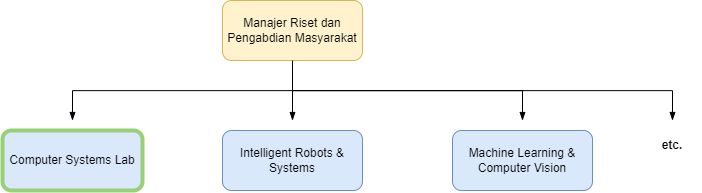
\includegraphics[width=1\textwidth]
	{assets/pics/pacil-org.png}
	\caption{Struktur Organisasi Pusat Penelitian Fakultas Ilmu Komputer UI}
	\label{fig:pacil-org}
\end{figure}

Dijelaskan pada \pic~\ref{fig:pacil-org} bahwa Computer Systems Laboratory (CSL) berada di bawah supervisi Manajer Riset dan Pengabdian Masyarakat, bersama dengan beberapa pusat penelitian lainnya, seperti Intelligent Robots \& Systems (IRoS) dan Machine Learning \& Computer Vision (MLCV). Struktur organisasi di CSL bersifat flat, di mana setiap penelitian dilakukan secara independen oleh masing-masing tim atau individu. Namun ada dosen peneliti yang bertanggung jawab memantau seluruh proyek untuk memastikan semua penelitian berjalan sesuai standar akademik.

Pelaksana kerja praktik ditempatkan dalam tim yang mengerjakan penelitian manajemen cluster Kafka, yang berfokus pada optimasi performa sistem distribusi data real-time. Sebagai \textit{Research Assistant}, pelaksana terlibat langsung dalam berbagai tahap eksperimen, mulai dari penyiapan infrastruktur hingga analisis hasil.
